\RequirePackage{luatex85}
\documentclass{standalone}

\usepackage{fontspec}
\usepackage{bm}

\usepackage{tikz}
\usetikzlibrary{arrows.meta}
\usetikzlibrary{decorations.text}
\usetikzlibrary{fit}
\usetikzlibrary{shapes.multipart}

\begin{document}
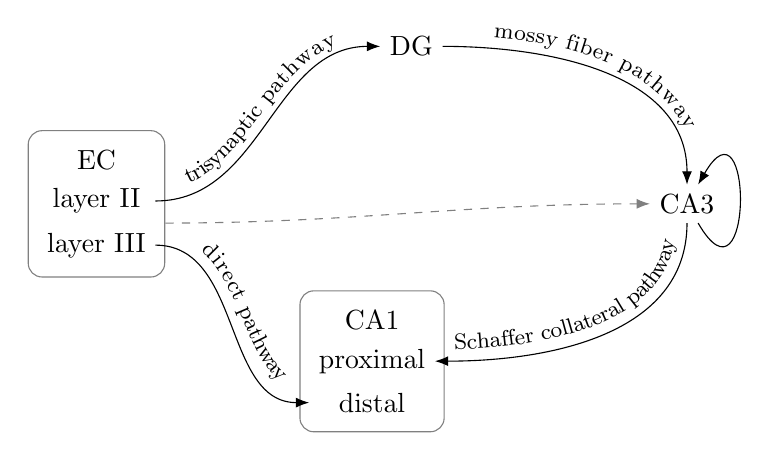
\begin{tikzpicture}[every path/.style={-Latex}]
    \node (ec) [rectangle split, rectangle split parts=3, at={(0, 0)}] {EC\nodepart{two}layer II\nodepart{three}layer III};
    \node (ec-outer) [draw, rounded corners=0.5em, gray, fit=(ec)] {};
    \node (dg) [at={(4, 2)}] {DG};
    \node (ca3) [at={(7.5, 0)}] {CA3};
    \node (ca1) [rectangle split, rectangle split parts=3, at={(3.5, -2)}] {CA1\nodepart{two}proximal\nodepart{three}distal};
    \node (ca1-outer) [draw, rounded corners=0.5em, gray, fit=(ca1)] {};

    \draw (ec.two east) to [out=0, in=180] (dg);
    \draw (dg) to [out=0, in=90] (ca3);
    \draw (ca3) to [out=270, in=0] (ca1.two east);
    \draw (ec.three east) to [out=0, in=180] (ca1.three west);
    \draw [gray, dashed] (ec.two split -| ec-outer.east) to [out=0, in=180] (ca3);
    \draw (ca3) to [out=300, in=60, distance=40] (ca3);

    \draw [decorate, decoration={text along path, text={|\footnotesize|trisynaptic pathway}, text align={center}, raise=4pt}, -{}] (ec.two east) to [out=0, in=180] (dg);
    \draw [decorate, decoration={text along path, text={|\footnotesize|mossy fiber pathway}, text align={center}, raise=4pt}, -{}] (dg) to [out=0, in=90] (ca3);
    \draw [decorate, decoration={text along path, text={|\footnotesize|Schaffer collateral pathway}, text align={center}, raise=4pt}, -{}] (ca1.two east) to [out=0, in=270] (ca3);
    \draw [decorate, decoration={text along path, text={|\footnotesize|direct pathway}, text align={center}, raise=4pt}, -{}] (ec.three east) to [out=0, in=180] (ca1.three west);
\end{tikzpicture}
\end{document}
